%%%%%%%%%%%%%%%%%%%%%%%%%%%%%%%%%%%%%%%%%
% AgroEV sketch
% 2017SoE027 
%
% Author: bmarron
% Origin: 28 Feb 2017
% Final:
%
% INSERT doc content into "ARTICLE CONTENTS" 
% MODIFY the "TITLE SECTION"
% MODIFY path references for all figures
%%%%%%%%%%%%%%%%%%%%%%%%%%%%%%%%%%%%%%%%%



%----------------------------------------------------------------------------------------
%	PACKAGES AND OTHER DOCUMENT CONFIGURATIONS
%----------------------------------------------------------------------------------------

\documentclass[twoside]{article}	%use

\usepackage{lipsum} % Package to generate dummy text throughout this template
\usepackage{csquotes}
\usepackage[natbibapa]{apacite}
\usepackage[english]{babel}
\usepackage{amsmath}
\usepackage{amsthm}
\usepackage{amssymb}
\usepackage{pdfpages}
\usepackage{verbatim}
\usepackage{bigfoot}
\usepackage{multirow}


\usepackage[sc]{mathpazo} % Use the Palatino font and the Pazo fonts for math
\usepackage[T1]{fontenc} % Use 8-bit encoding that has 256 glyphs
\linespread{1.05} % Line spacing - Palatino needs more space between lines
\usepackage{microtype} % Slightly tweak font spacing for aesthetics

\usepackage[hmarginratio=1:1,top=32mm,columnsep=20pt]{geometry} % Document margins
\usepackage{multicol} % Used for the two-column layout of the document
\usepackage[hang, small,labelfont=bf,up,textfont=it,up]{caption} % Custom captions under/above floats in tables or figures
\usepackage{booktabs} % Horizontal rules in tables
\usepackage{float} % Required for tables and figures in the multi-column environment - they need to be placed in specific locations with the [H] (e.g. \begin{table}[H])
%\usepackage{hyperref} % Interferes with cite.sty 

%\usepackage{lettrine} % The lettrine is the first enlarged letter at the beginning of the text
\usepackage{paralist} % Used for the compactitem environment which makes bullet points with less space between them

\usepackage{abstract} % Allows abstract customization
\renewcommand{\abstractnamefont}{\normalfont\bfseries} % Set the "Abstract" text to bold
\renewcommand{\abstracttextfont}{\normalfont\small\itshape} % Set the abstract itself to small italic text

\usepackage{titlesec} % Allows customization of titles
\renewcommand\thesection{\Roman{section}} % Roman numerals for the sections
\renewcommand\thesubsection{\arabic{subsection}} % Arabic numerals for subsections
\titleformat{\section}[block]{\large\scshape\centering}{\thesection.}{1em}{} % Change the look of the section titles
\titleformat{\subsection}[block]{\large}{\thesubsection.}{1em}{} % Change the look of the section titles

\usepackage{fancyhdr} % Headers and footers
\pagestyle{fancy} % All pages have headers and footers
\fancyhead{} % Blank out the default header
\fancyfoot{} % Blank out the default footer
\fancyhead[R]{\date{\today}}
\fancyfoot[R]{\thepage} % Custom footer text
%\fancyhead[C]{Running title $\bullet$ November 2012 $\bullet$ Vol. XXI, No. 1} % Custom header text
%\fancyfoot[RO,LE]{\thepage} % Custom footer text

%----------------------------------------------------------------------------------------
%	TITLE SECTION
%----------------------------------------------------------------------------------------

\title{\vspace{-15mm}\fontsize{14pt}{10pt}\selectfont\textbf{AgroEV: A LANDIS-II Extension to Evaluate the \\
Ecological Viability of Agroecological Landscapes}} % Article title

\author{
\large
\textsc{Bruce D. Marron} \\ %\thanks{A thank you or further information}\\[2mm] % Your name
\normalsize Portland State University \\ % Your institution
\vspace{-5mm}
}
\date{}

%----------------------------------------------------------------------------------------
\begin{document}
\maketitle                % Insert title
\thispagestyle{fancy}     % All pages have headers and footers

%----------------------------------------------------------------------------------------
%	ABSTRACT
%----------------------------------------------------------------------------------------

%\begin{abstract}

%end{abstract}

%----------------------------------------------------------------------------------------
%	ARTICLE CONTENTS
%----------------------------------------------------------------------------------------

This document is a sketch. It outlines the desiderata, the conceptual framework as primary assumptions, and the basic implementation mechanisms for a new extension for LANDIS-II termed, "AgroEV." 

\section{Desiderata for AgroEV}
The AgroEV extension should:
\begin{enumerate}
  \item \textit{Evaluate the process of agriculture through the lens of agricultural-ecological patterns and designs in the context of the mechanisms of agricultural-ecological mutualism} -- AgroEV must be able to discriminate between agricultural practices (temporal and spatial designs) based on fundamental ecological relationships between belowground soil food webs and aboveground net primary productivity. 
  \item \textit{Define a new algorithm for modeling the linkage between soil biodynamics and ecosystem processes that explicitly accounts for soil food web functionality and biodiversity} -- AgroEV must be able to incorporate concepts and understandings about plant-soil microbe relationships in such a way that while recent advances in rhizospheric biodynamics can be specifically acknowledged, future states of knowledge will not be excluded. That is, the AgroEV algorithm must be designed for updates, readily incorporating new states of empirically-derived knowledge about plant-soil microbe relationships.
\end{enumerate}


\section{Conceptual Framework}
The following "one-liners" provide the conceptual framework for AgroEV. They are are synthetic statements presented as a bulleted list of primary assumptions derived, in part, from this set of references:\\

\noindent \citep{ingham_interactions_1985}, \citep{maeder_soil_2002}, \citep{polis_food_1996}, \citep{van_der_heijden_unseen_2008}, \citep{lavelle_faunal_1997-1}, \citep{kladivko_tillage_2001}, \citep{doran_soil_2000-1}, \citep{bongers_nematode_1999}, \citep{brussaard_soil_1998}, \citep{coleman_peds_2008}, \citep{sackett_linking_2010}, \citep{kardol_how_2010},\citep{van_der_putten_empirical_2009}, \citep{bardgett_belowground_2014}, \citep{scheller_forest_2004}, \citep{williams_simple_2010}, \citep{fath_ecological_2007}, \citep{harte_maximum_2011}, \citep{gianinazzi_impact_1994}, \citep{eigen_hypercycle_1979}, \citep{nicolis_exploring_1989}

\begin{itemize}
  \item Plants are "super-organisms" composed of the autotroph and its rhizospheric symbionts. There are massive feedback loops between the autotroph and its symbionts governed by large numbers of biological transducers.
  
  \item Rhizospheric symbionts are species-rich communities of fungi and bacteria that feed directly from plant root exudates. These fungi and bacteria form the mutualisms that are the basis for a soil's rhizospheric-based soil food web component. 

  \item The rhizospheric-based soil food web component is a set of species-rich communities of fungi, bacteria, protozoa, and nematodes. The rhizospheric-based soil food web component is linked to the soil's detritus-based soil food web component, likewise a species-rich set of communities of fungi, bacteria, protozoa, and nematodes. Together, these two individual food web components form one, reticulate and mutualistic whole (the soil food web) with highly complex topology and population dynamics.
  
  \item Homogeneous trophic levels do not exist in soil food webs although temporal distance from photosynthetic carbon can define soil food web typologies: Rhizospheric-based communities are $10^{1} - 10^{3} \ s$ from photosynthetic carbon, detritus-based communities are $ > 10^{3} \ s$ from photosynthetic carbon.  
  
  \item Powered by photosynthetic carbon, soil food webs are complex adaptive systems maintained far from thermodynamic equilibrium. Soil food webs (and their plant allies) are Darwinian systems with virtually unlimited evolutionary potential. The evolutionary potential of soil food webs is the foundation for predicting the ecosystem scale effects of global change.
  
 \item Soil food webs drive nutrient recycling, soil formation, and soil fecundity. Plant health and productivity in natural systems depend on the diversity and viability of communities of (aerobic) soil microbes. Generally, soil biology drives soil chemistry, not the reverse.
 
  \item Soil food web processes directly affect patterns of landscape succession through variations in fungal/bacterial/protozoa/nematode ratios.
  
  \item The greater the structural and functional similarity of an agroecosystem to the natural ecosystems in its biogeographic region the greater the likelihood that the agroecosystem will be sustainable. 
  
  \item Sustainable agriculture is defined as ecological-agricultural mutualism -- the set of complex linkages, relationships, and practices that provide for mutually beneficial transfers of matter, energy, and information between the agriculturally-organized and the naturally-organized components of a multi-functional landscape. 
  
  \item Ecological-agricultural mutualism maintains biodiversity and evolutionary potential.

\end{itemize}


\newpage
\section{Implementation}
The implementation of AgroEV will require new inputs and new functionals for LANDIS-II.  Inputs can be direct measures, literature values, or best-estimates. A concept drawing of the AgroEV extension is shown in Figure 1 below.\\

%----------------------------------------------
\noindent \textbf{\underline{Current LANDIS-II inputs}}
%------------------------------------------------
\begin{enumerate}
  \item $a_1$ = Cell area (m)
  \item $a_2$ = Stand area (cells)
  \item $a_3$ = Ecoregion area (cells)
  \item $a_4$ = Plant species  (list)
  \item $a_5$ = Plant species life history data (per spp.)
  \item $a_6$ = Basic soil edaphics (per ecoregion)
  \item $a_7$ = Initial cohorts configuration (per cell)
\end{enumerate}

\vspace{5 mm}

%-------------------------------------------
\noindent \textbf{\underline{New AgroEV inputs}}
%-------------------------------------------
\begin{enumerate}
  \item $b_1$ = Biomass counts of soil fungi and soil bacteria ($\mu g / g$ per seral stage per stand)\footnote{Initially, the ratio of soil fungi:soil bacteria will be used as a proxy for soil food web functionality. This may need revision to include the ratio of protozoa:nematodes.)} 
  \item $b_2$ = Concentrations of $Na^{+}, \ Ca^{2+}, \ Mg^{2+}$ (meq/mL soil water extract per ecoregion)
  \item $b_3$ = Cation exchange capacity of mineral soil particles (non-organics only) (meq/100g dirt per ecoregion)
  \item $b_4$ = Depth to a compacted soil layer (or bedrock) (m per stand)
\end{enumerate}

\vspace{5 mm}

%------------------------------------------------------------------------------------------------------
\noindent \textbf{\underline{Spatially-explicit time series data currently generated by LANDIS-II}}
%-------------------------------------------------------------------------------------------------------

\begin{enumerate}
  \item $c_1$ = Species and age (cohort per cell per time)
  \item $c_2$ = Net primary productivity (per cell per time)
  \item $c_3$ = Biomass; aboveground (per cell per time)
\end{enumerate}


\vspace{5 mm}

%-------------------------------------------------------------------------------------------------------------------
\noindent \textbf{\underline{New, spatially-explicit time series data to be generated by AgroEV}}\\
%--------------------------------------------------------------------------------------------------------------------

\noindent \textit{F-series (Mappings1)}
\begin{enumerate}
  \item $F_1$ = Volume of root mass (per cell per time) = $f(a_1, a_4, a_5, b_3, b_4, c_1, c_2)$
  \item $F_2$ = Soil adsorption ratio (per stand per time) = $ {\frac {Na^{+}}{\sqrt {{\tfrac {1}{2}}({Ca^{2+}+Mg^{2+}})}}}$ = $f(b_2)$
  \item $F_3$ = Shannon diversity index for R species (per cell per time) = $-\sum _{i=1}^{R}p_{i}\ln p_{i}$ = $ f(c_1)$
  \item $F_4$ = Biomass; belowground (per cell per time) = $ f(c_2, G_4) $ 
\end{enumerate}

\noindent \textit{G-series (Mappings2)}
\begin{enumerate}
  \item $G_1$ = Rhizospheric density (per cell per time) = $f(F_1, adjacent \ cells)$\footnote{Adjacent cells are from the Moore neighborhood (\verb!http://mathworld.wolfram.com/MooreNeighborhood.html!)}   
  \item $G_2$ = Diversity of photosynthetic carbon inputs; root exudates (per cell per time) = $f(F_3)$
  \item $G_3$ = Diversity of photosynthetic carbon inputs; litter (per cell per time) = $f(F_3, adjacent \ cells)$
 \end{enumerate}  
  
\noindent \textit{H-series (Mappings3)}
\begin{enumerate}  
  \item $H_1$ = Soil food web cohort; a joint, conditional probability distribution (per cell per time) = $ Prob \ (Fungi, Bacteria | G_1, G_2, G_3)$
  \item $H_2$ = The maximum probability of the ratio of soil fungi:soil bacteria, X. The random variable, X is determined by first transforming the soil food web cohort distribution into a new probability distribution of soil fungi:soil bacteria ratios.  Five probability bins are then defined and X selects the bin containing the maximum amount of probability. A second random variable, W assigns a Greek letter as,  
 \end{enumerate}

\[ W = \begin{cases} 
      \alpha  & if \ 0\leq x_{MAX} \leq 0.3  \ (Pioneers) \\
      \beta  & if \ 0.3 < x_{MAX} \leq 1 \ (Early \ seral) \\
      \gamma  & if \ 1 < x_{MAX} \leq 5 \ (Young \ forest)\\
      \delta & if \ 5 < x_{MAX} \leq 100  \  (Mature \ forest)\\
      \epsilon & if \ 100 < x_{MAX}  \ (Old \ growth \ forest))
   \end{cases}
\]

\vspace{5 mm}

%------------------------------------------------------------------------------------
\noindent \textbf{\underline{AgroEV Outputs for Evaluation of Sustainable Ag }}\\
%-------------------------------------------------------------------------------------
\begin{enumerate}
  \item $O_1$ = Soil cation exchange capacity (per cell per time) = $f(b_3, G_4)$
  \item $O_2$ = Productivity index (per cell per time) = $ \frac{Total \ biomass \ accumulated \ in \ the \ system}{Net \ primary \ productivity}$ = $ f(c_2, c_3, F_4)$
  \item $O_3$ = Sequence of Greek symbols generated by the discrete random variable, W  (per cell per time).
\end{enumerate}


\section{Notes}
 The AgroEV extension is designed so that the "leak" of natural soil food webs into agricultural areas can be investigated as a "tweak" on sustainable production. That said, the implementation of AgroEV is not trivial. This is especially true of many of the mapping functions, many of which are speculative at this point. Ideally, threshold values for AgroEV outputs ($ O_1, O_2, O_3$) can be determined (per specific landscape) and used to evaluate regional-scale designs and practices for sustainable agriculture.

\begin{figure}
  \begin{center}
    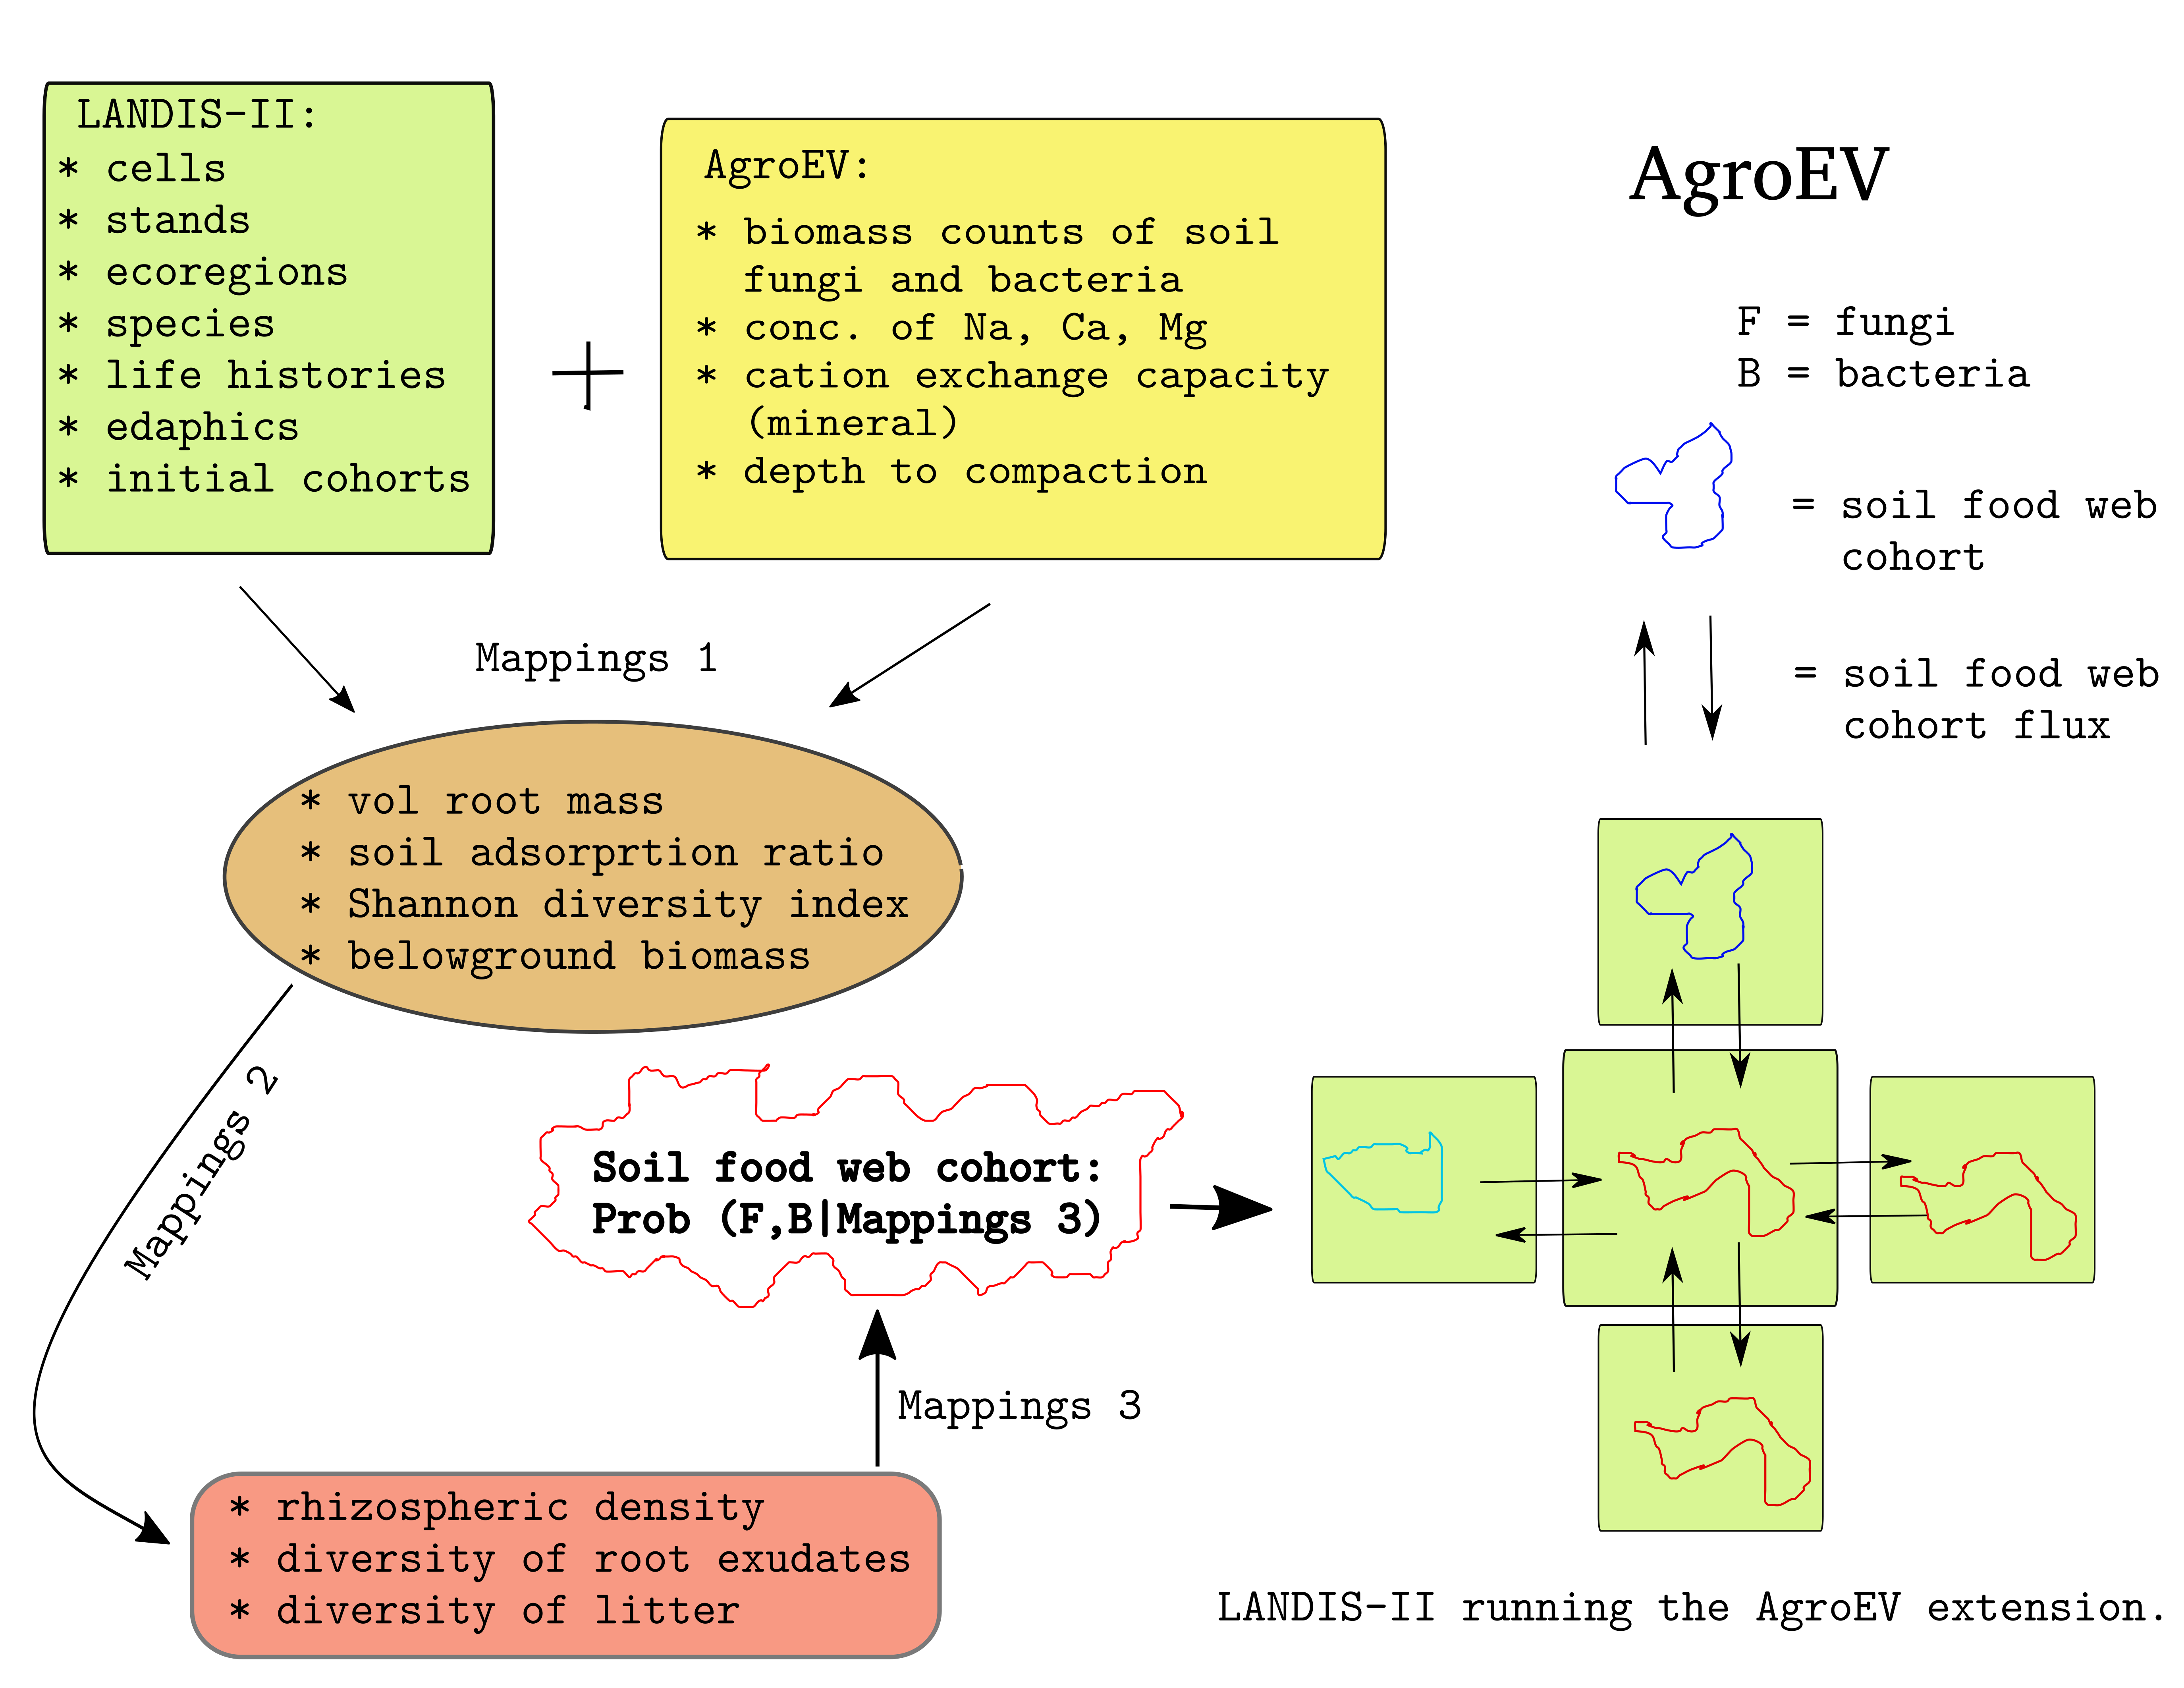
\includegraphics[scale = 0.60]{graphics/AgroEV_doc.png}
    \caption{Concept sketch of the AgroEV extension for LANDIS-II.}
    \label{fig:}
  \end{center}
\end{figure}



%----------------------------------------------------------------------------------------
%	REFERENCE LIST
%----------------------------------------------------------------------------------------
\newpage
\bibliographystyle{/usr/local/share/texmf/tex/latex/apacite/apacite}
\bibliography{/home/bmarron/Desktop/BibTex/My_Library_20170125}


\end{document}
